
%(BEGIN_QUESTION)
% Copyright 2006, Tony R. Kuphaldt, released under the Creative Commons Attribution License (v 1.0)
% This means you may do almost anything with this work of mine, so long as you give me proper credit

Hvor stort trykk blir pålagt dette U-rørsmanometeret med vann, målt i ``cm vannsøyle'' og ``Pascal''?

$$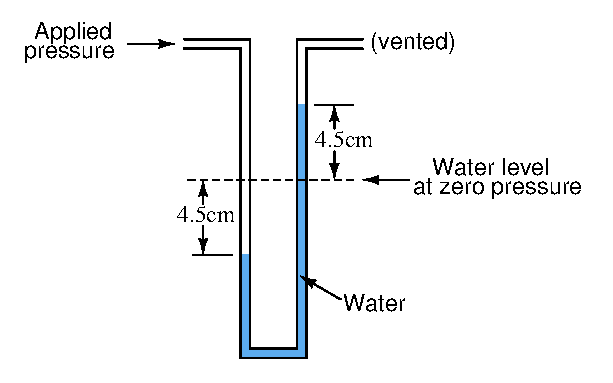
\includegraphics[width=15.5cm]{i00161x01.eps}$$

Hva ville skjedd med væskenivåene hvis vannet ble byttet ut med en olje med lavere \textit{tetthet}?  Ved samme pålagte trykk, ville avstanden mellom de to væskesøylene blitt større, mindre eller den samme som i figuren over?

\underbar{file i00161}
%(END_QUESTION)





%(BEGIN_ANSWER)

Pålagt trykk = 9 cm vannsøyle, som er lik 88.29 Pa

\vskip 10pt

Ved samme pålagte trykk vil avstanden mellom de to væskesøylene bli \textit{større} enn med vann.  Med andre ord: ved et trykk på 9" vannsøyle vil den vertikale avstanden mellom de to væskesøylene bli \textit{mer} enn 9 tommer.

I praksis virker manometre etter prinsippet om balanserte trykk: det pålagte gasstrykket tvinger væskesøylene til å forskyve seg i høyde.  Når de gjør det, dannes et hydrostatisk trykk som er proporsjonalt med høydeforskjellen.  Når dette hydrostatiske trykket er likt det pålagte trykket, stopper bevegelsen og systemet er i likevekt.

Hvis en lettere væske som olje brukes i stedet for vann, må en større høydeforskjell utvikles for å gi samme hydrostatiske mottrykk og oppnå likevekt.  Omvendt: hvis en tyngre (tettere) væske som kvikksølv brukes, vil en mye mindre vertikal høydeforskjell oppstå mellom søyler ved samme trykk.

%(END_ANSWER)





%(BEGIN_NOTES)


%INDEX% Measurement, pressure: manometer

%(END_NOTES)
